\chapter{Biomimicry: Nature as a Model}\label{ch:biomimicry}
\chapterauthor{jhanvi XXX}


\section{Biomimicry: Infastructure and Design Theory}

\subsection{Introduction}
Have you wondered how we have created submarines that can move so naturally through water? How the fastest train in the world travels at 200 miles per hour? How we have made needles that hurt less and less when you need to get that vaccine? The answer is that we have learned from nature.

This chapter explores the topic of Biomimcry, where it has been derived from and what it means, and then will focus on two case studies in the field. The chapter adds to the existing literature and scholarly conversation by focusing on learning from nature in Asia. 

Asian cultures have a rich history of learning from nature from medicinal plants to physical architecture of temples and pagodas they have all found inspiration outdoors. In the modern day, this connection is sometimes forgotten and my paper will try to re-bridge this. 

I will delve into the theoretical study of the subject and then suggest implementable solutions that are biologically inspired. The reason this is unique is because often times papers are limited to theory, and not actionable items and that is why my cases are supported by published patents, books, and even quotes from researchers who have capitalized on the science. 

My first case study, to be applied in China, explores the cement industry and how it can be changed to be more cost and energy effective, based on research conducted by a Stanford researcher. My second case study, to be applied in LA, explores how a design implemented in Beijing can be brought back to LA in designing an energy efficient stadium. 

Finally, we apply Biomimcry in Smart Cities and current examples of what exists, and what has worked and not worked, to understand the future of this field.

\section{What is Biomimicry?}
Biomimicry is an innovative approach to problem-solving, seeking sustainable solutions to human challenges, which emulate nature's time-tested patterns and strategies. This is developed based on the ideas that gave rise to chaos theory and fractal theory and others, which says that nature has already solved many of the problems which we are grappling with. The `secrets of survival' are becoming more and more important to humans as we progress technologically, and have fewer resources available. Biomimcry enables us to tap into this secrets, and harness them to make efficient and practical solutions.

\section{The Theory}

In order to understand how to apply Biomimcry, it is first essential to understand the theory that supports the field.\footnote{better, but you should have some text to help the reader understand what you are doing here}

\begin{enumerate}
  \item Function and Strategy\footnote{I think this/these should be subsections}
  

Biomimcry focuses on how nature, and living things, address certain functions or solve certain problems instead of how beautiful the solutions look, or how simple they are. A function is the purpose of a product or solution. In the context of biomimicry, function refers to the role played by an organism's adaptations or behaviours that enable it to survive. Functions can be met by systematic use of a system or a strategy. A biomimicry strategy is one that is a mechanism or process performing the function. It is often an adaptation to an environment where the function is needed. For example, the function of a honeybee is to collect nectar/ create honey for its honeycomb and for sustenance. The honeybee's strategy is to pollinate trees in the process of collecting nectar, and using its long snout to collect the nectar.
This section leaves us with two take-aways:
  \begin{itemize}
\item Ask yourself, what should my design do? 
\item Ask how questions. Eg: How does nature keep animals warm?
  \end{itemize}



  \item The Systems Perspective
When different functions and different solutions work together to impact a larger function, a system is created. The key thing here is the relationships between the smaller functions � if these are broken then none of the parts can serve their functions. As Buckminster Fuller once said, ``A system is greater than the sum of its parts.'' Systems have boundaries that allow the larger system to be broken into smaller ones or sub-systems. Many large systems can also connect to create super-systems. An example is the water system, the air system, and more create the processes that maintain nature's balance. Adjacent systems can exist at any of these levels, but influence similar systems and may have similar functions.

\item Earth's Operating System
The earth has physical boundaries which we can't leave easily. We are bound by our need for oxygen, by the atmosphere, and by the blanket of space surrounding us.
In this operating system, anything that imposes scarcity on the earth, shapes the system:

\begin{itemize}
  \item limited water
  \item limited air/ atmosphere
  \item limited sunlight, from which all energy ultimately is derived
  \item gravity
  \item biological systems that have been shaped around these scarcities
  \item competition and predation which led to evolution as a system of sustenance
\end{itemize}

\item Natural Patterns

Natural patterns include things that are persistent, and don't regularly change. Examples of this include:
\begin{itemize}
  \item Natures ability to recycle everything it produces
  \item Natures ability to use shape as a mode of function
  \item Natures inherent feedback loops- ability to change when something goes wrong
\end {itemize}

\end{enumerate}

\section{Biomimicry as a worldview}

Biomimicry is a unique way of looking at any topic. It accepts that fundamentally everything in nature has a function and a strategy. It is similar to systems thinking such that the natural environment is its system, and everything within it is interdependent. As explained in the section above, finding the function of a system or product is the first step in making the connection between the object, what it is used to accomplish, and how it accomplishes the task. 
	
A function, by definition, is the purpose of something. In the context of biomimicry, function refers to the role played by an organism's adaptations or behaviours that enable it to survive. Here is a list of functions that are underlying most natural tendencies and can be found in objects and tasks:

\begin{itemize}

\item Attach or Move
  \begin {enumerate}
    \item Move or Stay put
    \item Protect from Physical Harm
    \item Protect from living things
    \item Protect from non-living threats
    \item Manage structural forces
    \item Regulate physiological processes
    \item Prevent structural failure
  \end {enumerate}

\item Maintain Community
  \begin {enumerate}
    \item Coordinate
    \item Cooperate
    \item Provide Ecosystem Services
  \end {enumerate}

\item Modify
  \begin {enumerate}
    \item Modify Physical state
    \item Modify chemical/ electrical state
    \item Adapt/ optimize
    \item Transform/ convert energy
  \end{enumerate}

\item Make
  \begin {enumerate}
    \item Reproduce
    \item Physically assemble
    \item Chemically assemble
  \end{enumerate}

\item Process Information
  \begin{enumerate}
    \item Navigate
    \item Send signals
    \item Process signals
    \item Sense Signals/ environmental cues
    \item Compute/ learn/ de or en-code
  \end{enumerate}

\item Break down
  \begin{enumerate}
    \item Chemically break down
    \item Physically break down
  \end{enumerate}

\item Get, Store, or Distribute Resources
  \begin{enumerate}
    \item Capture, Absorb, or filter
    \item Store
    \item Distribute
    \item Expel
  \end{enumerate}
  
\end{itemize}

\section{Biomimcry History}

Biomimicry as a pedagogy was developed\footnote{developed seems like the wrong word} first in 500 B.C when the Greeks saw biological organisms as models in finding harmonious balance and proportion between the parts of a design that is synonymous to classical ideal of beauty. This was used as inspiration in finding the Golden Ratio or 2.16 which is the ratio of plant stems to petal length, or bird wingspan to body. The Golden Ratio came to be a defining beauty standard, and normalised the comparison of natural and man-made objects. In 1482, Leonardo Da Vinci was inspired by birds flying to invent a flying machine. This is an early example of Biomimicry. This also helped in the development of the Wright's brother first prototype to make an airplane in 1948. In 1958, Jack E. Steele introduced the term Bionics and he defined it as the science of natural systems or their analogues.  However, the term Biomimicry itself first appeared in 1982 before which it was an abstract concept. In 1997, scientist and author Janine Benyus popularized the term more in her book, ``Biomimicry: Innovation inspired by Nature'' . In 2005, Bryony Schwan and Janine Benyus co-founded the Biomimicry 3.8 and in 2007 Chris Allen joined Beynus and Schwan to help launch ``AskNature'' which is the first digital library containing a list of natural solutions to global problems. Scientists argue that Biomimicrt picked up traction after nano-engineering became popular in the 1990s. Here, designers can search a collection of natural systems classified by their design and engineering. Today for example, look at the nose design of Japan's speedy bullet trains and how they resemble a bird's beak. Biomimcry is continually growing but can sometimes exist in academic bubbles. For a solutions based pedagody like this to exist and get better, it needs to be exposed to geographic differences and perspectives. 

%\insertphoto

\begin{figure}
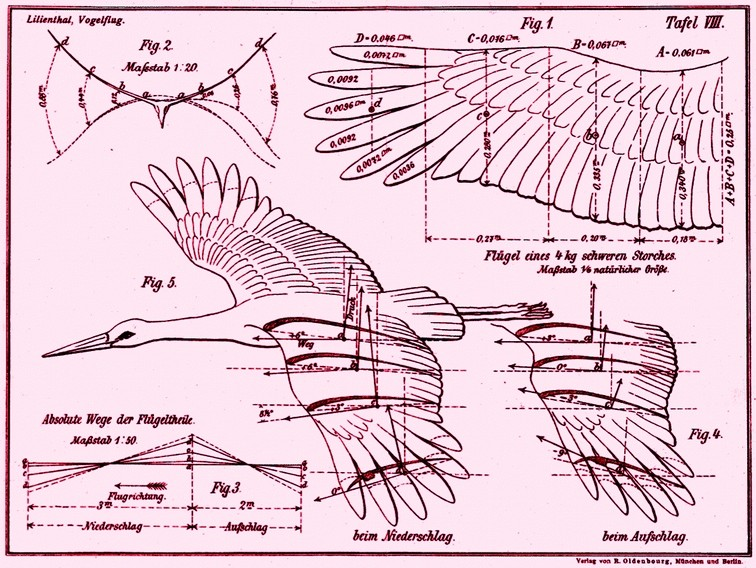
\includegraphics[width=\textwidth]{new_feature}
\caption{Drawings inspired by birds, used in designing the first flying machines}
\label{fig:news_featured}
\end{figure}

\section{Case Study: The Cement Industry alternatives}

In order to best see how far we have come in the applications of Biomimcry, we can look at examples within industries of its applications. Biomimicry application in the cement industry has been one of interest to many scientists because it is an industry on which human progress is based. We urbanize, and sustain large populations, by building structures out of cement. In addition, it is an industry that contributes hugely to the world GDP, and uses a lot of energy. Because both the outcomes and inputs in this system are huge, any solutions could revolutionize the future. Let us turn to China which is a prime example of a robust system.
China, in the last three years, has used more cement than the United States in the 20th century.  Cement production has been uniform for several years, and is often inefficient and unsustainable. How does cement production take place? What are its uses? How can this problem can be solved using a biomimicry approach? How is this different in impact than before?

Cement is eventually used to make concrete, so we will cover only the production of cement in this section. There are two ways to produce cement which are covered in the next two subsections.

\subsection{Dry Process}

1.	Quarry the principal raw materials - limestone, clay, and others. This is followed by crushing the rock, first to a 6 inch size, then using hammer mills to reduce the pieces to 3 inches or smaller.
2.	The crushed rock is combined with other ingredients such as iron ore or fly ash and ground, mixed, and fed to a cement kiln.
3.	The cement kiln heats all the ingredients to about 2,700 degrees Fahrenheit in huge cylindrical steel rotary kilns lined with special firebrick. Kilns are mounted with the axis inclined slightly tilted away from the horizontal to avoid settling.
4.	The finely ground raw material or the slurry is fed into the higher end. At the lower end of the kiln, there is a flame produced by controlled burning of powdered coal, oil, alternative fuels, or gas. During this movement in the kiln, some gases are given off, and the remainder unites to form a new substance called clinker. Clinker comes out of the kiln and is discharged red-hot from the lower end of the kiln.
5.	The heated air from the coolers is returned to the kilns, a process that saves fuel and increases burning efficiency. The clinker is then cooled, cement plants grind it and mix it with small amounts of gypsum and limestone. 

\subsection{Wet Process}

In the wet process, raw materials are ground with water before being fed into the kiln between steps 2 and 3.

\subsection{Characteristics of the Cement Industry}

Cement is used as the main binding element in concrete, used for constructing bridges, roads, buildings, and many other man-made sites. It is a construction material used for decoration and for practical purposes but its large-scale production influences the way we look at emissions and carbon economies.
Cement production needs a lot of energy, and is CO2 and raw materials intensive. Even these raw materials being quarried or produced require energy. Any changes to the cement production processes will reduce this amount of energy consumed. The combination of process emissions (emissions released when limestone is transformed into lime during the production process) and emissions from the required thermal energy leads to substantial CO2emissions for each tonne of cement. 

In addition to the environmental costs, cement production has significant economic costs.  Building a cement plant costs hundreds of millions of dollars. In addition, making sure that the plant is complying with all the legislation and operation costs also makes this an expensive field. 30 percent of the cement industry's total operating expenses relate to energy costs. The cost of a new cement plant is equivalent to around three years of turnover, which ranks the cement industry among the most capital-intensive industries. 

Cement is interesting because it must be a homogenous product. It is made from the same natural ingredients each time but must meet a standard because it can otherwise have many safety breaches. This standard makes the market high in competition if some plants can produce the outcome at cheaper costs in cheap labour markets like China. Many developed countries import cement from countries like China for this reduced cost. Transporting cement across countries, or from plants to construction sites, also poses a major energy consumption outcome.
The Cement Industry, because it is tied to construction, is a good indicator of general economic activity. When a country is booming, and economy is growing, there are more infrastructure and developmental projects ongoing. 

Connecting it back to the theory of Biomimcry, the solutions for the cement industry were derived from corals. Corals in the open ocean are solid structures made from calcium carbonate where organisms live and thrive. Their function, similar to cement, is to remain solid and to organize people and space. In addition to this, cement also has an economic function where the organization of people and space earns a lot of money.

All these factors make it essential for us to find sustainable solutions for this industry.

\subsection{The Biomimcry Solution}

The biomimicry solution for cement is based on inspiration derived from the formation of Coral reefs. Instead of consuming carbon dioxide, this method actually removes Carbon dioxide from the environment which we talked about earlier as one of the big problems with this industry. This method was found by Brent Constantz of Stanford University, who founded the company Calera. The method takes waste CO2 from local power plants and dissolves it into seawater to form carbonate, which mixes with calcium in the seawater and creates a solid.  This is the same way that corals form skeletons and we can create cement.

Constanz has described this method in the following way. There is a natural interaction between CO2, which is a gas, and water. At equilibrium, the CO2 is dissolved in water. The colder the water is, the more CO2 is dissolved into it. This forms another molecule, CO3, or carbonate. The higher the concentration of CO2, the more carbonate formed. When water interacts with very high concentrations of CO2, like the flue gas of a power plant, more CO2 is dissolved in water to form carbonate. 
At Calera, there is a 110 foot high absorber, a vertical carwash, which is spraying sea water through a big, vertical column. At the base of the column comes the flue gas from this power plant. It comes up from the base of the column, and it goes up and goes over the top. On its way out, with the sea water spraying through it, the same reaction occurs. The CO2 goes to CO3 as it dissolves in the water.
Sea water has calcium. When the calcium sees the carbonate, calcium carbonate is formed. This is the same as limestone is, and how corals form their shells. Solids formed from this process look like milk and fall to the bottom of the column to be separated. They're dried out using the waste heat from the hot flue gas. To trap the heat of the hot flue gas, a heat exchanger is used so there is no burning of fossil fuel to dry it out. This produces a powder in a spray dryer, which is akin to a machine making powdered milk. This is the cement. The cement can be used to make aggregate, synthetic rock like synthetic limestone, or it can be kept dry as a cement and used in a concrete formulation.

%\insertphoto
\begin{figure}[h]
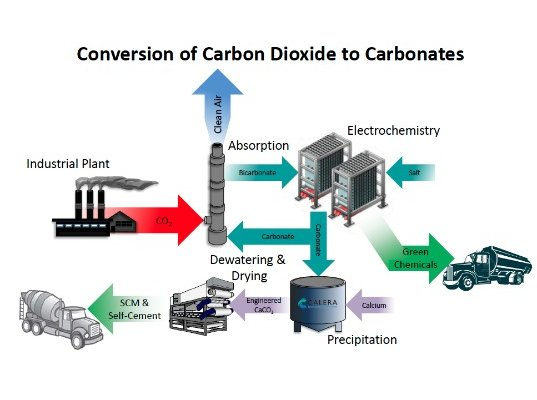
\includegraphics[width=\textwidth]{Calera-Carbonate-Technology-1}
\caption{How Calera technology forms Cement using Biomimcry}
\label{fig:Calera-Carbonate-Technology-1}
\end{figure}

This process captures CO2, waste heat and fly ash from power plant smokestacks, and runs the CO2 through seawater to produce calcium carbonate to make cement. This unique process has distinct outcomes that solve for some of the problems we discussed earlier. The flue gas out of the kiln (step 4) is cleaned of its harmful CO2. In addition, carbon is sequestered in the cement which then balances out the further carbon production from mining and transportation of cement. The seawater remaining at the end is also pre-treated for desalination for drinking water and has more use than it did before.  

The problem with this method is that it asks for the cement production technique to be completely changed. This means that all the capital investment in the industry so far is wasted, and will require new investments to change the status quo. Keeping this in mind, there is a different biomimicry approach that can be taken.

This approach uses bacteria to repair cracks in concrete and it is a more reactive approach instead of a pre-emptive one to the problem of inefficiencies in concrete production.  As populations continue to rise and current buildings and structures are used to their maximum, this approach might be beneficial in reducing concrete waste and thus reduced overproduction. If 25\% of total waste in Europe comes from construction and demolition, according to Eurostat, a similar number may be modelled in China and other parts of Asia.  This bacteria based option is inspired by the ability of octopi to regrow their lost tentacles, by Dutch microbiologist and finalist of the 2015 European Inventors award, Hendrik Jonkers.
Jonkers includes, in traditional and non-traditional concrete, natural bacteria (bacillus pseudofirmus and B. cohnii) capable of producing limestone.  These bacteria are normally dormant but are put into action when they come into contact with water which flows through cracks on a structure. Then, limestone fills the cracks. In addition, the bacteria are aerobic and so they consume oxygen within the confines of the structure. This reduces the amount of internal corrosion of metal in the structure. The bacteria can remain dormant for even up to 200 years which means that even long-term impact can be made in these major civil engineering projects. This reduces maintenance costs, and lowers resource consumption in making new structures.

This idea is being explored by several scientists with different bacteria and substances over the world. One such example is found in a paper by Vijay, Murmu and Deo,  where urease engendering bacteria along with the introduction of a calcium source can result in calcite precipitation in cement. Bio-mineralization techniques, like this one, seal natural and time-created cracks. These are permanently sealed by a perpetual hydration process. The ureolytic bacteria, suggested to be used, includes Bacillus Pasteurii, and Bacillus Subtilis which can engender urea along with the calcium source to seal the freshly composed micro cracks by CaCO3 precipitation. This paper, amongst others, shows that the use of bacteria can increase the strength and durability properties of concrete. This may be seen as retrofitting of cement.

\subsection{Cost-Benefit Analysis}

Assumptions
-	Cement making industry is expensive but required for the production of materials that have a lot of uses
-	The process uses energy that is not clean, and imposes a cost on the environment
-	Its expenses cannot be paid off if a cement manufacturing plant is used for a short period of time
-	Energy consumption is bad because of the production of greenhouse gases during the energy manufacturing, and this leads to rising temperatures on the planet
Discount rates
-	The cost of producing cement is already expensive, but the fact that it can be stored over time leads to the cost depreciating such that the dollar could have been used elsewhere. Instead the money is used for excess production and more money is used to transport it to assure appropriate allocation of the good.
Externalities
-	The Biomimicry system of making concrete has the unintended consequence of desalinating seawater for other uses in the world. This is a positive externality
-	The retrofitting option reduces oxygen within the concrete structure which reduces corrosion of the steel and other metals used in a building structure
Flaws
-	This may reduce the import money coming into China from cement production because countries will begin to make their own cement at low maintenance rates.
How is system improved by Biomimicry
-	Reduced energy use because reduced cement production leads to reduced GHG emissions and reduced impact on global warming
-	The second system allows infrastructure projects to last longer and for casualties of human life to be reduced because bridges and buildings are less likely to collapse if cracks are immediately repaired by bacteria

\section{Case Study: Applying Asia's innovation to the United States}

It is often assumed that the East learns from the West and from the 'civilized world' but learning from the natural environment has been a big part of the Eastern culture, historically. This ranges from Ayurveda and ancient medicine, to building dung houses to keep cool in the same way that animals use mud/dung. This section explores the reverse - a Biomimcry solution applied in the east which has potential to be brought back. An example of this in Vietnam is the way that local use the leaves of water coconuts, which are waterproof and have the ability to float. The locals sew them together to make roofs that protect their homes from rainfall.

\begin{figure}[h]
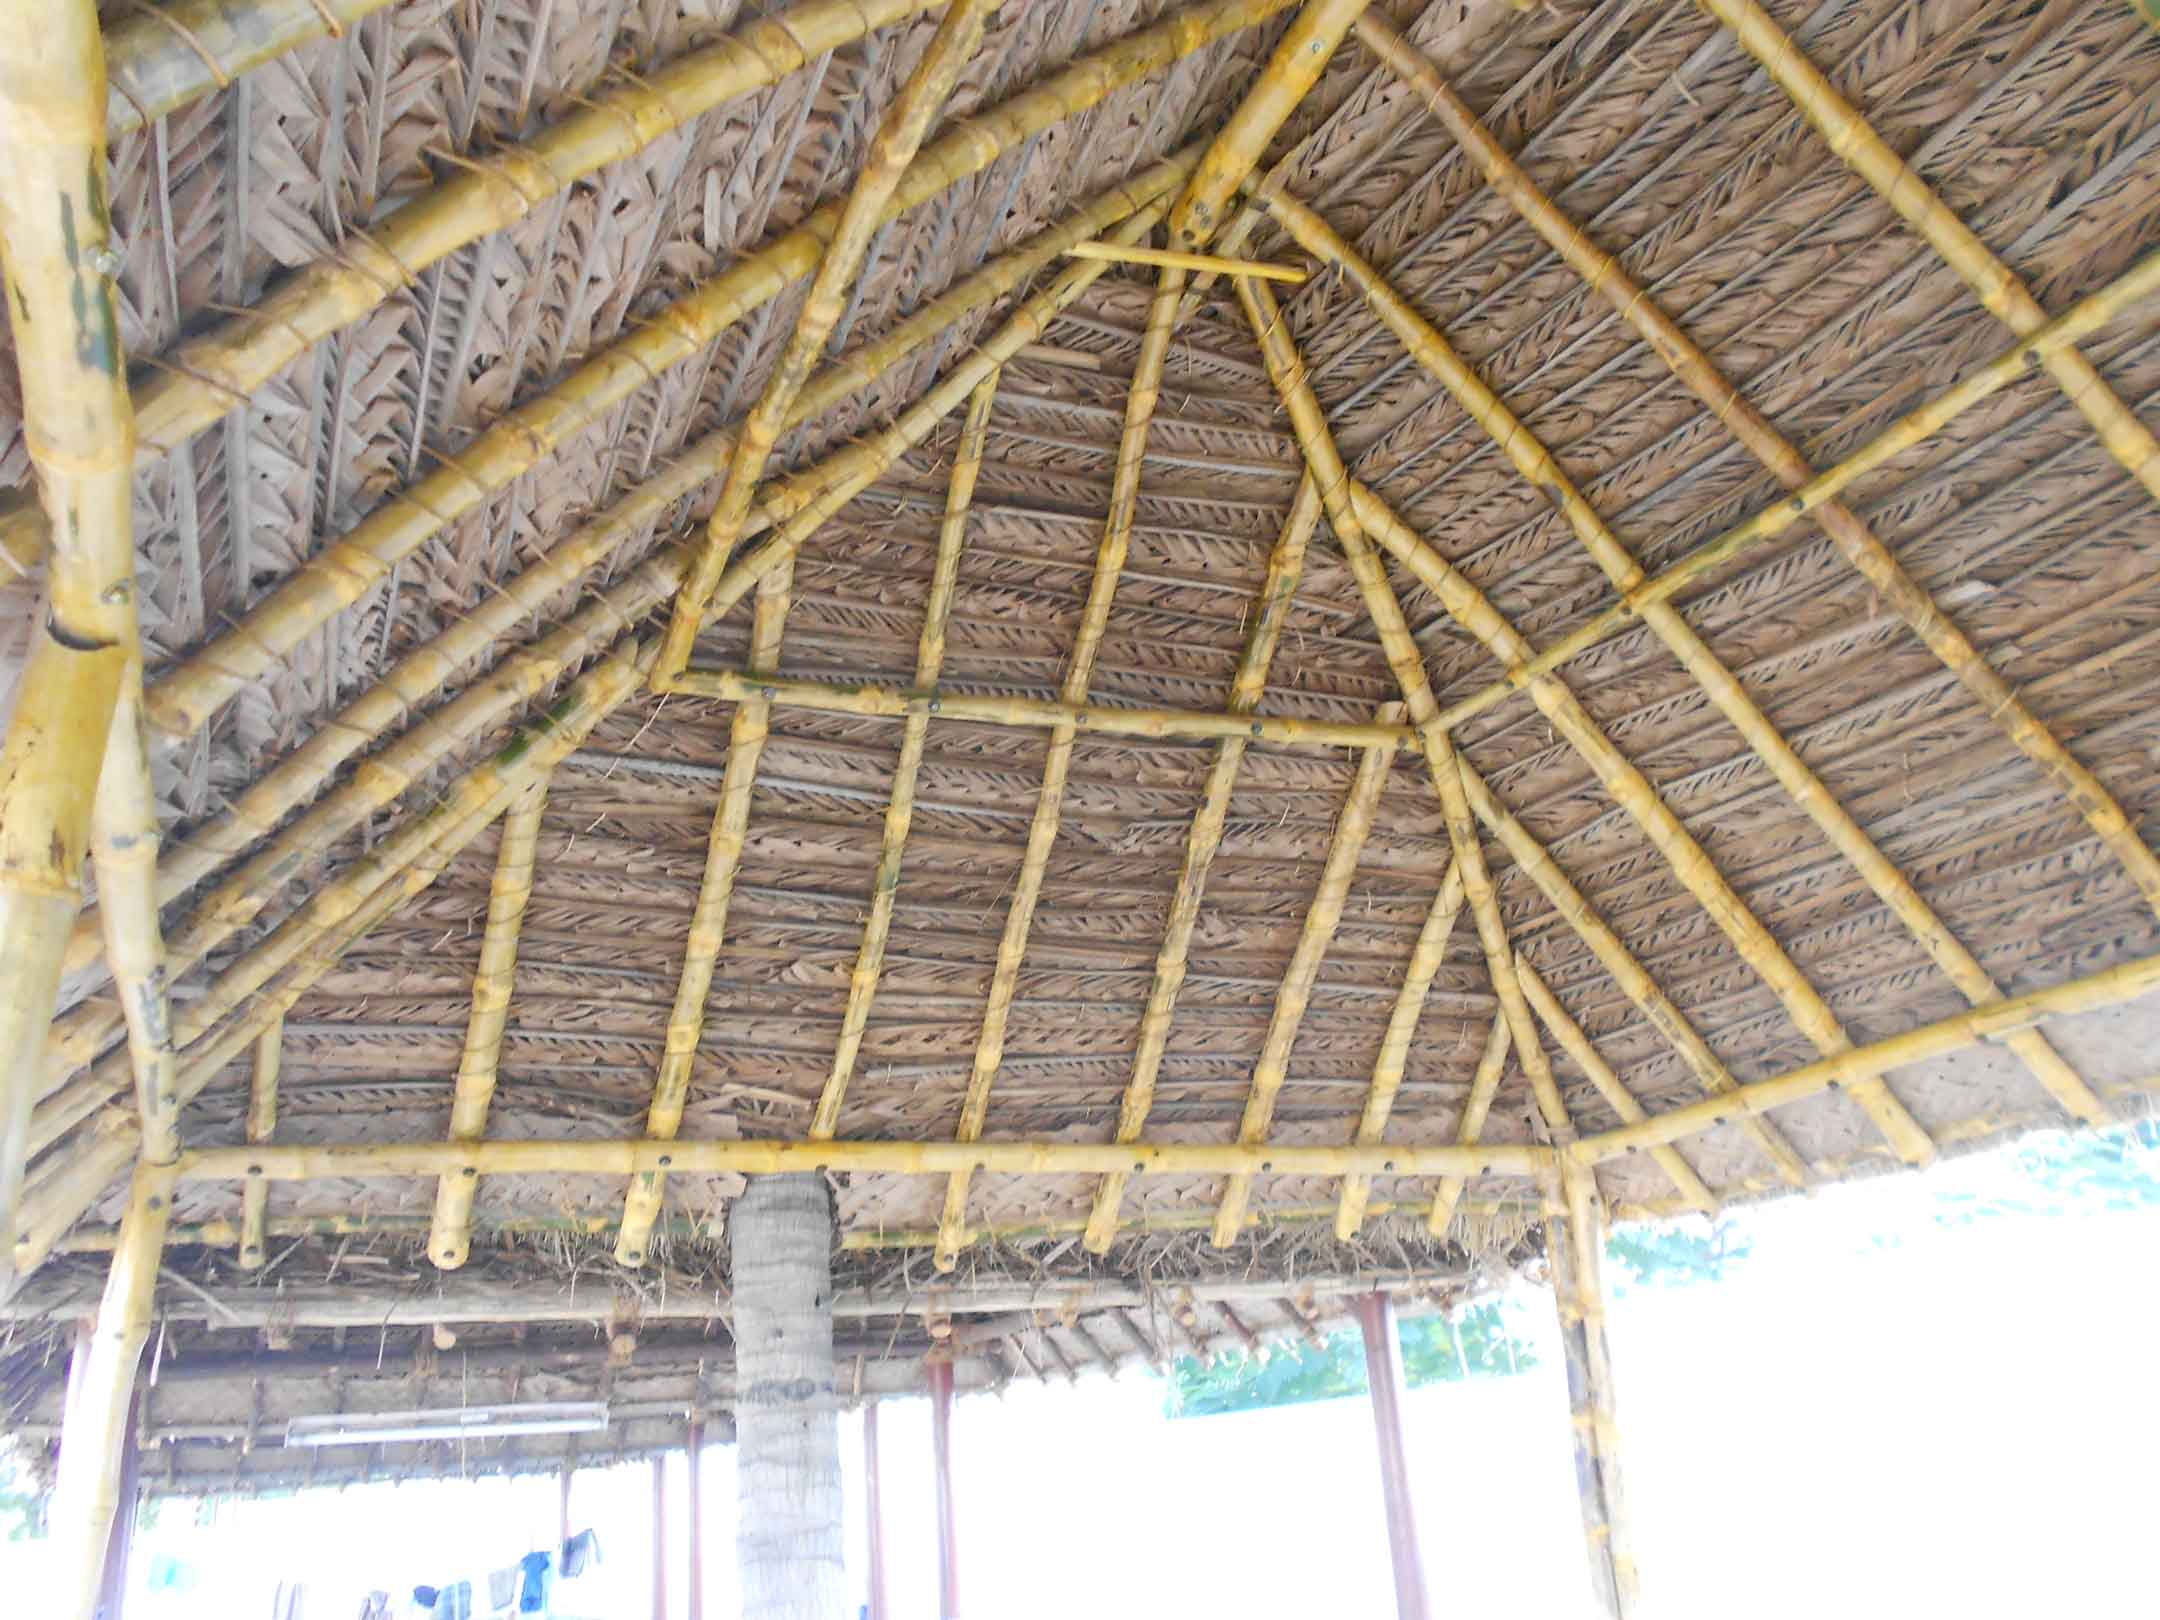
\includegraphics[width=\textwidth]{Coconut-Leaf-Thatching}
\caption{some caption}
\label{fig:Coconut-Leaf-Thatching}
\end{figure}

\subsection{Characteristics of infrastructure industry}

Stadiums are an important point of focus, and have a lot of value in the field of Biomimcry because of the role of ``infrastructure'' as a glamorous industry. While infrastructure can sometimes be thought of as dry and functional, bridges, stadiums, and some other structures stand as testament to those attracting tourists and investments and attention. Examples of this include the Eiffel tower, and more locally, the Golden gate bridge. In addition, the industry employs millions of people at all its different stages --- from energy, to cement production, to labor and manufacturing. This way, it engages large populations. Applying biomimicry to this space would allow this large population to value this field of education and allow publicity of a valuable takeaway--- we are always learning from nature. Infrastructure can become a balance of technical progress, of human kind's power, alongside nature's mastery of systems.

\subsection{The Bird's Nest Stadium as a Biomimcry Solution}

This study is based on the Bird's Nest Stadium or Beijing's National Stadium, which staged the 2008 Olympic games, but has been proven to be innovative yet energy efficient.  The stadium is designed by Swiss architects Herzog \& de Meuron, inspired by Asian history which I will talk about further. The stadium took five years to complete and was constructed using 42,000 tons of steel, making it the largest steel structure in the world. 

Here are the basic features that make the stadium comparable to any other stadium to be built in the future:

\begin{itemize}
  \item A stadium capacity of approximately 100, 000 people 
  \item A retractable roof, 
  \item A multi-functional design to incorporate different performances and games in the future 
The structure is famous because it is the largest volume of steel used in a project like this - the structure encloses steel approximately 333 meters long by 284 meters wide and 69 meters tall. It must be noted that Steel is easily recyclable and these smaller ``green'' initiatives were intentional by the architects.
\end{itemize}

%\insertphoto

\subsection{Applying Bio-infrastructure to Los Angeles}

The Bird's Nest Structure, and similar bioinspired structures may be applicable in Los Angeles because this structure was designed to withstand earthquakes without much damage because it is originally located in one of the world's most seismic zones. The Bird's Nest Stadium can withstand an 8.0 magnitude earthquake. A part that may be easier to figure out in LA, than in Beijing, is the effect of thermal expansion. In Beijing, the temperature can range from over 30�C in the summer to -20�C in the winter, and the architects had to account for this tendency of steel to expand and contract as the temperature changes. LA, like temperature is more uniform yet warmer than in many places where such structures have been built. It is time to think - what are local metals that can be used? How different are the social needs in LA and Beijing? Perhaps, with LA being an upcoming green corridor, with increasing interest in organic foods and trends, such infrastructure will create a domino effect so locals are inspired to make a change. There is an underlying social component to Biomimcry which is how it makes a public statement for people to recognize how we have eliminated nature from our day-to-day, and also how we have opportunities to incorporate nature effectively if we are more conscious.

See Figure~\ref{fig:aerial_view}.

\begin{figure}[h]
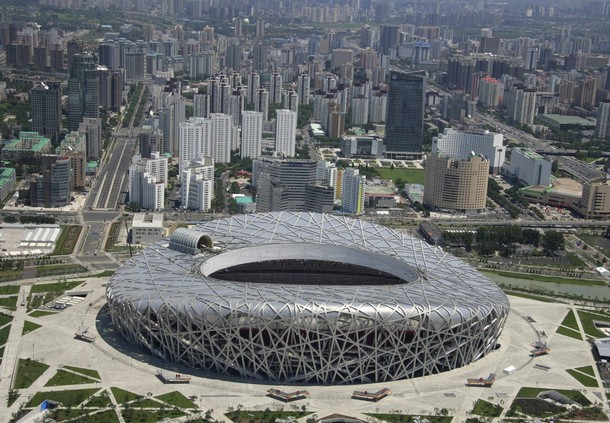
\includegraphics[width=\textwidth]{aerial_view}
\caption{some caption}
\label{fig:aerial_view}
\end{figure}

\section{Biomimicry and Smart Cities}

As population sizes grow bigger, and the rural-urban diaspora grows larger, the need for efficient use of space and energy grows more imminent. In this case, natural spaces also grow smaller and people are concerned about finding ways to be in nature. More and more studies find that natural settings and trees increase productivity, and access to this is increasingly cut off in cities. This section will tackle how we can better intertwine nature in cities without humanly recreating nature and destroying its sanctity. Then it will tackle the role of biomimicry in creating smart cities and the role of automation in these cities. 

Cities are interesting, especially in asia, because they pose the large challenge where they host large portions of the country's GDP, and the country's population, but are becoming increasingly polluted and hard to live in. This problem becomes a desperate one to solve in order to get some of these countries to move from developing to developed.

An example of smart evolution in cities is being developed by Cambridge bioengineer Michelle Oyen who has been making artificial bone and eggshells. Now, her samples are only centimeters in length, but one day they make up high-rises and skyscrapers. One of the big natural case studies scientists are trying to recreate is the problem of tree cover. In the built environment, when the site is cleared and the vertical structure is taken out or land is left barren, rain directly hits the ground at maximum velocity. In forests, especially virgin forests like those remaining in some parts of Borneo, the ecosystem is structured with the shrub layer, the mid-level tree layer, and the canopy layer. All these layers slow down the rain so that by the time it actually hits the soil it is absorbed very quickly.

Biomimcry may also be used to have better transportation networks across cities. When automation changed things so that people used `cars' instead of horses, it influenced the culture of the world in more ways than was predicted. Cars come with a culture around racing, around transportation and consumption of goods produced all over the world/ country, around the mindset that the place you live is not the only place you know. It led to the tourism and travel industry, the booming of economy and trade, and more. It can be predicted that smarter transportation may transform the world in similar ways. 

Arndt Pechstein is a neuroscientist in Berlin who is working on a project inspired by this concept. He is working with researchers at the Audi Urban Future Initiative to rethink Berlin's transportation network and he is inspired by the way ``cargo'' moves within the cells of our bodies.

Proteins and organelles---the ``cargo''---are transported via carriers called motor proteins that travel along different microtubules, or ``streets.'' He describes in an interview how a single motor protein is not only able to carry one specific cargo, so it can be decoupled from that cargo to take on another r. He also describes how there are different motor proteins that can switch between different infrastructures without any waiting time or delay.  Here is a diagram showing this idea.

%\insertphoto

\begin{figure}
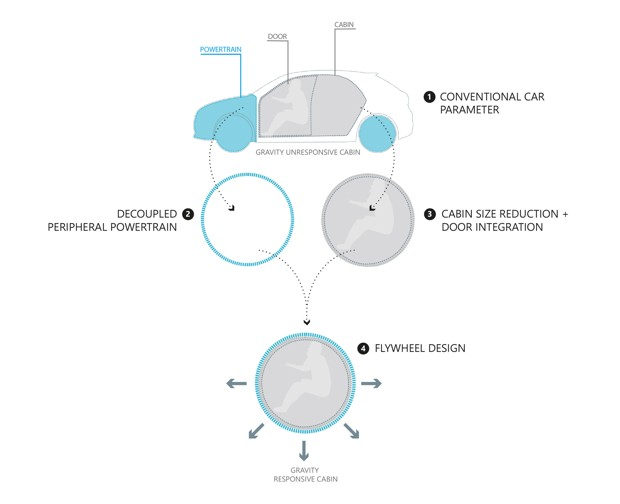
\includegraphics[width=\textwidth]{1720d6946}
\caption{some caption}
\label{fig:1720d6946}
\end{figure}

Smart cities, with efficient transportation, and efficient energy usage, and space for millions of people to live without waste accumulation, drought, or the creation of food deserts, require sustainability efforts. These smart cities are also sometimes called Sustainable cities or Eco-cities. An eco-city, is first defined in 1987 by Richard Register in his book ``Ecocity Berkeley: building cities for a healthy future,''  as a city designed with consideration of environmental impact, inhabited by people dedicated to minimization of required inputs of energy, water and food, and waste output of heat, air pollution --- carbon dioxide, methane, and water pollution.  A city like this sustains little on surrounding suburbs and countryside. This means reduced transportation of goods and people into and out of the city, which leads to reduced car usage and pollution. This means different things for different industries. For agriculture, it means an investment in vertical farming, in low-land-use plants, in potentially genetically manufactured products. For energy production, it means solar panels, biomass energy plants, converting waste to energy, and other small-scale production. The Central Intelligence Agency estimates that 55 percent of total world population lives in Urban environments. This only makes our cause more urgent. Industrial ecology (IE), defined as a `systems-based, multidisciplinary discourse that seeks to understand emergent behaviour of complex integrated human/natural systems' is also the study of material and energy flows through industrial systems such as cities. There are many ways to study the application of Biomimcry to urban planning but this chapter will now follow initiatives that have already been taken in this field. 

\subsection{Existing initiatives in Asia}


It is important to go back to initiatives that have been successful to reflect on what works, and what can be done to make these better, in Asia and outside.
China, in partnership with the Singaporean government, is building an ecocity in the Coastal New District of Tianjin City in northern China, named the ``Sino-Singapore Tianjin Eco-city.'' The goal is that Tianjin Eco-city will support both countries in tackling environmental protection, resource conservation, energy conservation, and sustainable development, and serve as models for sustainable development for Singapore and other cities in China. Another such initiative is Rizhao. Rizhao, recognized by the United Nations as one of the most habitable cities in the world in 2009, is situated on the coastline along the Yellow Sea, and features a major seaport. The city mandates solar panels and solar water heaters in all new buildings, and oversees the construction process to ensure the panels are correctly installed.  The effort to install solar water heaters began in 1992. As of 2007, 99 percent of households in the central districts use solar water heaters, and most of the lighting and traffic signals are powered with photovoltaic solar power. In 2007 the city had over a half-million square meters of solar water heating panels, which have effectively reduced conventional electricity usage by 348 million kilowatthours per year. The city has been designated as the Environmental Protection Model City by China's SEPA, and is consistently listed in the top 10 cities for air quality in China.  The city population stands at 2,801,100 as of the 2010 census, and stands as a successful smart and sustainable city.

\subsection{Failed initiatives}

Failures are important to define successes, and find the things that are not socially acceptable, but are not actually adhering with natural convention. Following is an example of both.	Dongtan Eco-city is the name of the third largest island in China at the mouth of the Yangtze River near Shanghai. Dongtan was publicized as an urban center for green technologies and how smart design can cut the carbon footprint of up to a half-million people in the area. The project was scheduled to accommodate 50,000 residents by 2010, but its state-owned developer has currently put construction on hold.  Huangbaiyu is another major eco-city being built by China which is ready, but uninhabited. In 2003, Leading American ``green'' architect and designer William McDonough teamed with Deng Nan, to promote economically sustainable development in China through the China-US Centre for Sustainable Development. They hoped that Huangbaiyu would become an example of how technology could improve villagers' lives and reducing energy costs and consumption. This is a more rural solution with the village made of ``eco-dwellings`` or houses built from hay and pressed-earth bricks, which are fully insulated and solar-powered.   Such a unique project has become inspiration to many sociologists and anthropologists who hope to understand people who chose to partake in these spacial experiments. 

\subsection{Benefits of a Smart City}

Now that we have recognized smart cities and eco cities as places that use bio-inspiration in intersection with technology, it is important to assess how this would transform our lives socially and physically. This is interesting because intuitively, it might seem like nature and technology cannot coexist without one being rampant. The two ways this paper suspects smart cities and technology can coexist is by increasing government accountability, and data access.

Government accountability: A smart city has increased transparency, data collection and technology usage to track information. This reduces information asymmetry in the government and in public sector jobs where productivity and outcomes are not accurately measured. 

Data access. Accessible data creates opportunities for new private-sector services and companies that could potentially change residents' lives. This includes a popular example - transit information lends which can combine city, weather, and traffic data to help transit users decide whether a bikeshare, bus, or train is their best option on a given day.

\subsection{Risks of a Smart City}

There are drawbacks though, to compromising 'nature' where technology doesn't typically have a place. This paper suspects that the two aspects most affected will be privacy risks, and technology becoming a cover for ineffective reforms. 
Privacy risks: Data sharing and collection may lead to more personalised services and products, but this may also breach certain levels of privacy and even autonomy. Leaks of such data, especially in sensitive parts of the country's affairs, like the government, may be a risk that the country has to bear. Keeping data safe is a major area for research and development in an environment where the governments' ability for surveillance goes up, and civil rights and privacy are always under the spotlight.
Cover for ineffective reforms. Policy or Legal upholdings may be compromised by both politicians, lobbyists, and lawyers because they may lack the incentive to pursue these long term, meaningful changes. Instead, many changes will be technological solutions which are not guaranteed to have results, either positively or negatively.


\section{Conclusion}

Biomimcry is important because research in this field started off from a systems perspective. It started off as an attempt to design cleaner, faster, and better structures with efficiency and engineering in intention. Today, Biomimcry is changing as our moral responsibility as humans increases. There is value in assimilating with the natural environment, in going back to the ways that nature conducted processes and built structures. This value comes from sustainability --- reduced waste, reused materials, and organic materials. This value comes from bowing down to nature and submitting to its design tendencies --- learning from what exists. In many Asian cultures, nature is compared to god. God being the force that runs the world and created the world. Here, it seems Biomimcry would be well accepted for its moral outcomes. Then we are simply giving back to the Earth what we have taken from it. Pragmatically, it is accepted that both efficiency and sustainability goals might drive bio-inspiration, but it is important to accept the context of sustainability and how it helps us save the future of the world. 

This textbook talks about many morbid realities of the globe. It talks about palm oil deforestation, climate change in Thailand, soil erosion, changing food production in Korea, a breadth of research. Biomimicry brings to it all, a fresh perspective, and an opportunity for repair. Perhaps, there might be ways in which we cut down carbon emissions, and slow down climate change, by reducing cars in cities. We may be able to reduce soil erosion by creating building foundations that function like roots which retain water in the soil. Through this, Biomimcry is a solution-driven branch of Environmental Analysis. It is a young, yet promising field of study in a world which is simply driven by understanding problems and not brainstorming solutions. As students who have had the chance to visit Singapore, Vietnam, Thailand, India, travel across urban and rural spaces with local people, we have hope. We have hope that people still value each other, and value the earth as is. As the population continues to grow, and the earth is burdened with resource overutilization, it is imperative that we remember that humans have always learned and bounced back. This is our time, and Biomimcry is a tool we can use to restore what was once the glory of Earth.


\citep{benyus1997biomimicry}


\citet{china_ecovillage}

%\end{enumerate}
